\documentclass[10pt]{article}

\usepackage[margin=1in]{geometry}
\usepackage[T1]{fontenc}
\usepackage[utf8]{inputenc}
\usepackage{lmodern}
\usepackage{microtype}
\usepackage{graphicx}
\usepackage{subcaption}
\usepackage{booktabs}
\usepackage{tabularx}
\usepackage{array}
\usepackage{amsmath, amssymb}
\usepackage{siunitx}
\usepackage{enumitem}
\usepackage{xcolor}
\usepackage{hyperref}
\usepackage{tikz}
\usetikzlibrary{arrows.meta, positioning, fit}

\graphicspath{{figures/}{../experiments/plots/}}
\hypersetup{
  colorlinks=true,
  linkcolor=blue!50!black,
  citecolor=blue!50!black,
  urlcolor=blue!50!black,
}
\captionsetup{font=small}
\setlength{\parskip}{0.35em}
\setlength{\parindent}{0pt}
\sisetup{
  round-mode=places,
  round-precision=3,
  detect-weight=true,
  detect-family=true,
}

\title{\textbf{Attention-Augmented Scale Hyperprior for Learned Image Compression}}
\author{Emre Y{\i}lmaz \\ CS566 Deep Learning, Spring 2026}
\date{}

\begin{document}
\maketitle

\begin{abstract}
We investigated whether lightweight channel attention can improve learned image compression when added to a standard scale-hyperprior architecture. Starting from the official CompressAI implementation of Ball\'e et al.'s scale hyperprior, we implemented two Squeeze-and-Excitation (SE) variants: encoder-only attention and encoder+decoder attention. The hyperprior itself was kept unchanged so that the attention modules could be evaluated as a controlled architectural modification. Compared with the original proposal, the final training pipeline uses explicit CLIC train/validation image folders rather than DIV2K, and it adds a fine-tuned vanilla baseline to make the comparison fair.

Training was performed on 1,633 CLIC training images with 102 validation images using random 256$\times$256 crops, and evaluation was carried out on the 24-image Kodak benchmark. We report PSNR, MS-SSIM, estimated bitrate, and true coded bitrate obtained from actual \texttt{compress()}/\texttt{decompress()} calls. This distinction became important during project cleanup: earlier intermediate plots based only on estimated bitrate overstated the benefit of the SE variants, while the corrected coded-bitrate evaluation shows that the curves are nearly identical.

The final results do not support a meaningful rate-distortion gain from the tested SE modification. Relative to the fine-tuned vanilla baseline, encoder-only SE yields a PSNR BD-rate of \(+0.08\%\) and encoder+decoder SE yields \(+0.17\%\); the MS-SSIM differences are similarly negligible. Across the four operating points, the project variants stay within \(0.009\) dB and \(5.8\times 10^{-4}\) bpp of each other. In contrast, stronger entropy models such as MBT 2018 and Cheng 2020 provide much larger gains. Within the scope of this course project, the main conclusion is that small transform-side SE attention is easy to integrate, but it does not materially improve compression performance in this setting.
\end{abstract}

\section{Introduction}
Learned image compression replaces fixed transforms and hand-designed probability models with neural networks trained directly for rate-distortion optimization. This is attractive because the encoder, decoder, and entropy model can be adapted jointly to the data distribution rather than optimized as separate components. In recent years, learned compression models have become competitive enough that small architectural changes can be tested systematically, which makes them a good fit for a graduate course project.

The starting point of this project was the scale hyperprior model of Ball\'e et al.~\cite{balle2018hyperprior}, implemented through CompressAI~\cite{begaint2020compressai}. The original proposal asked a narrow question: if we keep the hyperprior unchanged and only add lightweight attention inside the transform network, do we obtain better rate-distortion behavior? This is a modest goal, but it is scientifically useful because it isolates the effect of the attention block from larger changes to the entropy model.

The final repository stays close to that plan at the model level. We implemented two attention-augmented variants: one with SE attention in the encoder and one with SE attention in both encoder and decoder. At the same time, the experimental pipeline evolved in two important ways. First, the final training runs use CLIC train/validation splits instead of the initially planned DIV2K training set. Second, we added a fine-tuned vanilla control baseline because comparing SE variants only against the frozen official pretrained model would not be a fair test of the modification.

This report therefore focuses on two questions. First, did the implementation correctly realize the proposed modification? Second, after using the corrected evaluation pipeline and fair baselines, do the SE blocks improve image compression on Kodak? The short answer is that the implementation is technically consistent with the proposal, but the experimental evidence for improvement is weak.

\section{Related Work}
Classical codecs such as JPEG and later transform-based codecs rely on carefully engineered transforms, quantization rules, and entropy coders. Their main strength is robustness and efficiency, but the transform and prior model are fixed in advance. Learned compression instead treats compression as a rate-distortion learning problem, allowing the transform and latent prior to adapt to the training distribution.

An early end-to-end formulation was introduced by Ball\'e et al.~\cite{balle2017e2e}, who showed that nonlinear transforms with a differentiable rate surrogate can be optimized directly. The scale hyperprior model~\cite{balle2018hyperprior} improved this idea by introducing a second latent variable \(z\) that predicts spatially varying scale parameters for the main latent \(y\). This hyperprior remains one of the standard baselines in learned image compression and is the backbone used in this project.

Subsequent work showed that stronger entropy models often matter more than modest changes in the analysis/synthesis transforms. Minnen et al.~\cite{minnen2018joint} combined a hierarchical prior with autoregressive context modeling and achieved clear gains over the scale hyperprior. Cheng et al.~\cite{cheng2020anchor} further improved the prior and also used attention-style components together with a discretized Gaussian mixture likelihood. These models are relevant here because they provide a reference for how much improvement can be expected from a stronger prior versus a lightweight transform-side modification.

Our approach is deliberately simpler than Cheng et al.~\cite{cheng2020anchor}. We do not change the entropy model, the latent dimensionality, or the likelihood family. Instead, we insert Squeeze-and-Excitation channel attention blocks~\cite{hu2018senet} into the transform network while keeping the hyperprior unchanged. This makes the comparison cleaner, but it also limits the expected gain. In hindsight, the final results follow the literature: stronger priors provide larger improvements than the small SE augmentation tested here.

\section{Data}
Table~\ref{tab:data-summary} summarizes the datasets present in the repository and clarifies which ones were used in the final runs.

\begin{table}[t]
\centering
\small
\caption{Datasets found in the repository and their final role in the project.}
\label{tab:data-summary}
\begin{tabularx}{\linewidth}{@{}l l c l l@{}}
\toprule
Dataset & Role & Count & Resolution & Final use \\
\midrule
CLIC train & training & 1,633 & variable & yes \\
CLIC validation & validation & 102 & variable & yes \\
Kodak PhotoCD & test benchmark & 24 & mostly \(768\times512\) & yes \\
DIV2K train & alternate train set & 800 & high-resolution & no \\
DIV2K validation & alternate val set & 100 & high-resolution & no \\
\bottomrule
\end{tabularx}
\end{table}

The proposal planned to train on DIV2K and evaluate on Kodak. The final implementation instead uses local CLIC image folders for training and validation. This change is visible both in the YAML configuration and the dataset loader used by \texttt{train.py}. The repository still contains DIV2K assets and a download helper, but they are not part of the final reported pipeline.

The preprocessing is simple and consistent with patch-based compression training. For training, each image is converted to RGB, reflect-padded if it is smaller than the patch size, randomly cropped to \(256\times256\), and randomly flipped horizontally. Validation uses the same patch size but replaces random cropping with a center crop. No per-channel normalization is applied beyond converting the image to a \([0,1]\) tensor. Kodak evaluation uses full-resolution PNG images; each image is reflect-padded to a multiple of 64 for the convolutional transforms, and metrics are computed only on the original unpadded region.

This pipeline is reasonable for a course project, but it has two limitations. First, there is no separate held-out CLIC test set in the final setup; Kodak is the only external benchmark. Second, because the model is trained with MSE loss but also reported with MS-SSIM, the MS-SSIM numbers should be interpreted as secondary evaluation rather than a directly optimized target.

\section{Methods}
\subsection{Baseline Model and SE Variants}
The baseline is the pretrained \texttt{bmshj2018\_hyperprior} model from CompressAI~\cite{begaint2020compressai}, corresponding to the scale hyperprior of Ball\'e et al.~\cite{balle2018hyperprior}. For an input image \(x\), the model computes
\begin{align}
y &= g_a(x), \\
z &= h_a(y), \\
\hat{z} &\sim p_{\hat{z}}, \\
\sigma &= h_s(\hat{z}), \\
\hat{y} &\sim p_{\hat{y}\mid \hat{z}}(\cdot \mid \sigma), \\
\hat{x} &= g_s(\hat{y}),
\end{align}
where \(g_a\) and \(g_s\) are the analysis and synthesis transforms, \(h_a\) and \(h_s\) form the hyperprior branch, and the latent likelihoods define the bitrate surrogate.

Our modification leaves \(h_a\), \(h_s\), the entropy bottleneck, and the Gaussian conditional unchanged. The only change is the insertion of Squeeze-and-Excitation (SE) blocks into the transform network. Given a feature map \(f \in \mathbb{R}^{C \times H \times W}\), the SE block computes
\begin{align}
s &= \sigma\!\left(W_2 \, \mathrm{ReLU}(W_1 \, \mathrm{GAP}(f))\right), \\
f'_{c,h,w} &= s_c \cdot f_{c,h,w},
\end{align}
where \(\mathrm{GAP}\) is global average pooling and \(s \in [0,1]^C\) rescales channels. Variant \(B\) inserts one SE block in the encoder after the second convolution; variant \(C\) inserts the same encoder block and one additional SE block in the decoder after the second transposed convolution.

\begin{figure}[t]
\centering
\resizebox{\linewidth}{!}{%
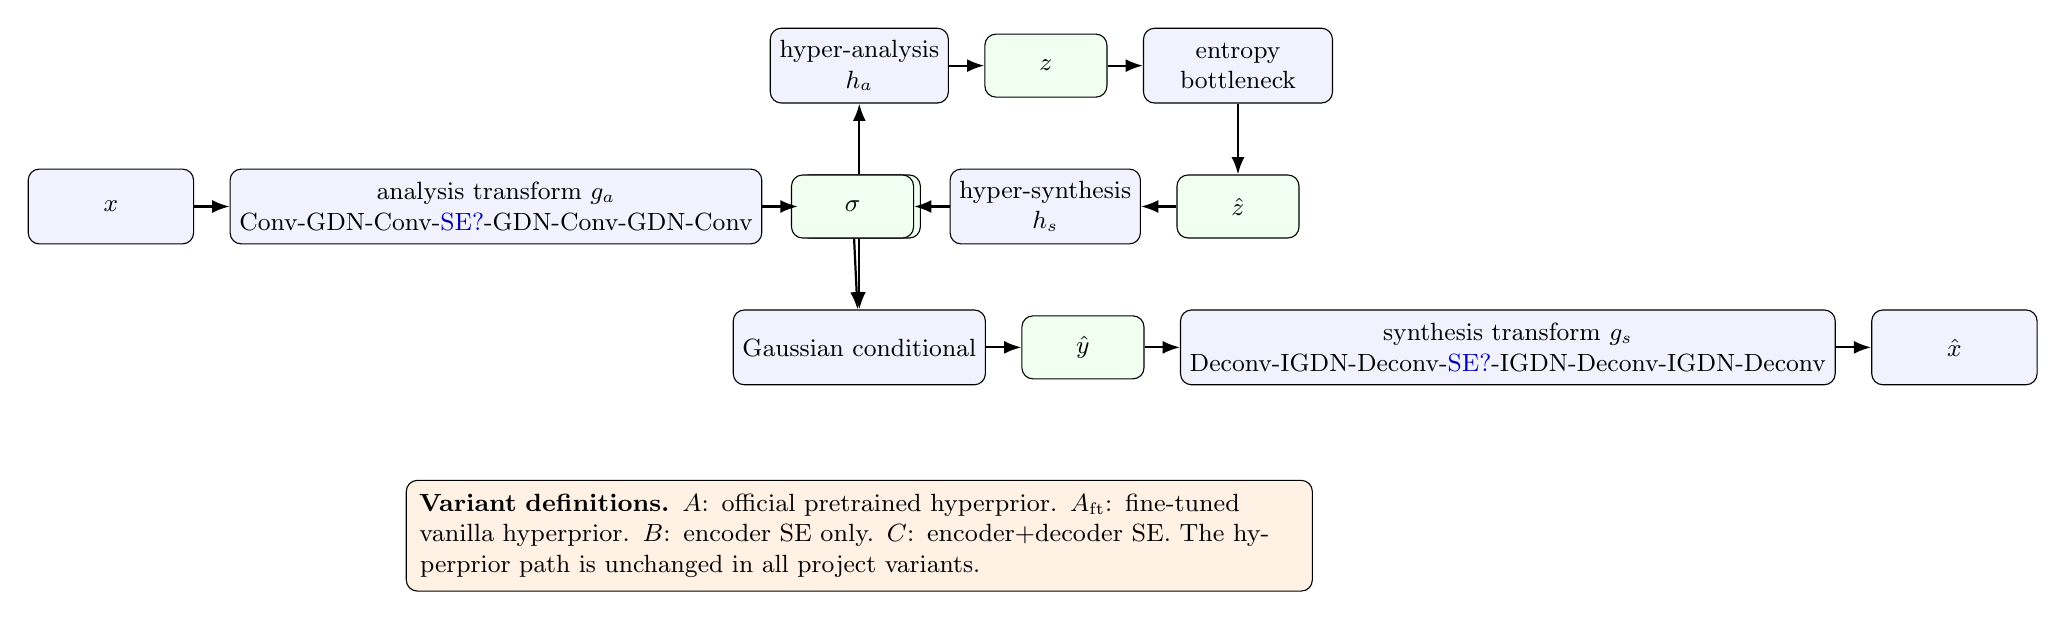
\begin{tikzpicture}[
  node distance=0.9cm and 0.45cm,
  box/.style={draw, rounded corners, align=center, minimum height=0.95cm, minimum width=2.1cm, fill=blue!5},
  latent/.style={draw, rounded corners, align=center, minimum height=0.8cm, minimum width=1.55cm, fill=green!6},
  note/.style={draw, rounded corners, align=left, fill=orange!10, inner sep=5pt},
  arr/.style={-{Latex[length=2.2mm]}, thick},
  font=\small
]
\node[box] (x) {\(x\)};
\node[box, right=of x, minimum width=2.9cm] (ga) {analysis transform \(g_a\)\\Conv-GDN-Conv-\textcolor{blue!70!black}{SE?}-GDN-Conv-GDN-Conv};
\node[latent, right=of ga] (y) {\(y\)};
\node[box, above=of y, minimum width=2.2cm] (ha) {hyper-analysis\\\(h_a\)};
\node[latent, right=of ha] (z) {\(z\)};
\node[box, right=of z, minimum width=2.4cm] (eb) {entropy\\bottleneck};
\node[latent, below=of eb] (zhat) {\(\hat{z}\)};
\node[box, left=of zhat, minimum width=2.2cm] (hs) {hyper-synthesis\\\(h_s\)};
\node[latent, left=of hs] (sigma) {\(\sigma\)};
\node[box, below=of y, minimum width=2.5cm] (gc) {Gaussian conditional};
\node[latent, right=of gc] (yhat) {\(\hat{y}\)};
\node[box, right=of yhat, minimum width=3.0cm] (gs) {synthesis transform \(g_s\)\\Deconv-IGDN-Deconv-\textcolor{blue!70!black}{SE?}-IGDN-Deconv-IGDN-Deconv};
\node[box, right=of gs] (xhat) {\(\hat{x}\)};

\draw[arr] (x) -- (ga);
\draw[arr] (ga) -- (y);
\draw[arr] (y) -- (gc);
\draw[arr] (y) -- (ha);
\draw[arr] (ha) -- (z);
\draw[arr] (z) -- (eb);
\draw[arr] (eb) -- (zhat);
\draw[arr] (zhat) -- (hs);
\draw[arr] (hs) -- (sigma);
\draw[arr] (sigma) -- (gc);
\draw[arr] (gc) -- (yhat);
\draw[arr] (yhat) -- (gs);
\draw[arr] (gs) -- (xhat);

\node[note, below=1.2cm of gc, text width=0.92\linewidth] {
\textbf{Variant definitions.}
\(A\): official pretrained hyperprior.
\(A_{\mathrm{ft}}\): fine-tuned vanilla hyperprior.
\(B\): encoder SE only.
\(C\): encoder+decoder SE.
The hyperprior path is unchanged in all project variants.
};
\end{tikzpicture}
}
\caption{Implemented architecture. The proposal's core idea is preserved: attention is added only to the transform network, while the entropy model remains the standard scale hyperprior.}
\label{fig:architecture}
\end{figure}

Figure~\ref{fig:architecture} shows the final architecture. The change is intentionally lightweight: at quality level 3, variant \(B\) adds only 2,184 parameters and variant \(C\) adds 4,368 parameters over the 5.08M-parameter baseline.

\begin{table}[t]
\centering
\small
\caption{Implemented model variants used in the report. Parameter counts come from the final evaluation summaries.}
\label{tab:variants}
\begin{tabularx}{\linewidth}{@{}l X c@{}}
\toprule
Variant & Description & Parameters \\
\midrule
\(A\) & Official pretrained scale hyperprior reference & 5,075,843 \\
\(A_{\mathrm{ft}}\) & Fine-tuned vanilla hyperprior control baseline & 5,075,843 \\
\(B\) & Encoder-only SE attention & 5,078,027 \\
\(C\) & Encoder+decoder SE attention & 5,080,211 \\
\bottomrule
\end{tabularx}
\end{table}

\subsection{Initialization and Optimization}
All project variants are initialized from the official pretrained scale hyperprior weights. For the SE variants, pretrained weights are transferred into the modified layer indices, while the new SE blocks are initialized near the identity: the second fully connected layer is initialized with zero weights and a bias of 5.0, so the initial sigmoid outputs are close to 1. This is a sensible engineering choice because it reduces the disruption caused by inserting new modules into an already trained compression model.

Training uses the rate-distortion objective
\begin{equation}
\mathcal{L} = \lambda D(x,\hat{x}) + R(\hat{y}) + R(\hat{z}),
\label{eq:rd}
\end{equation}
where \(D\) is MSE in the main experiments and
\begin{equation}
R = -\frac{1}{HW}\sum \log_2 p(\hat{y}) - \frac{1}{HW}\sum \log_2 p(\hat{z}).
\end{equation}
The implementation follows the standard CompressAI convention and scales the MSE distortion by \(255^2\). Four operating points are trained with \(\lambda \in \{0.0018, 0.0035, 0.0067, 0.013\}\), matched to quality levels 1--4.

Optimization uses Adam with separate learning rates for backbone and SE parameters: \(10^{-4}\) for pretrained backbone weights, \(10^{-3}\) for SE parameters, and \(10^{-3}\) for the auxiliary entropy-model quantiles. The scheduler is \texttt{ReduceLROnPlateau} with factor 0.1 and patience 10. Runs stop after 100 epochs at most, with early stopping after 20 epochs without validation-loss improvement. Batch size is 32, patch size is \(256\times256\), and training is deterministic with seed 42.

\subsection{Freeze-Mode Ablations and Evaluation Protocol}
Beyond the proposal, the final repository includes three training modes: \texttt{none}, \texttt{frozen\_hyperprior}, and \texttt{attention\_only}. The first updates all trainable weights, the second freezes the hyperprior path, and the third updates only the SE parameters. These ablations help answer whether the SE modules are useful as small adapters or only when the full model is allowed to adapt.

For evaluation, the repository computes both estimated bitrate from latent likelihoods and true coded bitrate from actual entropy coding. The final report uses true coded bitrate for all primary conclusions. This matters because the differences among \(A_{\mathrm{ft}}\), \(B\), and \(C\) are very small: for the project variants, coded bitrate exceeds estimated bitrate by only \(1.56\times 10^{-4}\) to \(1.10\times 10^{-3}\) bpp, but that is already comparable to the size of the observed gaps between the curves.

The final evaluation code also measures runtime. A forward pass is timed on the main CUDA model with synchronization before and after \texttt{model(x)}. True encoding and decoding times are measured separately using \texttt{compress()} and \texttt{decompress()} on a CPU copy of the model, because the entropy-coding path in CompressAI is CPU-based in this setup. We therefore report three timing numbers: forward time, encode time, and decode time, along with the codec total (encode+decode). These measurements are useful for testing the ``lightweight'' claim, but they should still be interpreted as machine-specific rather than universal throughput numbers.

\begin{figure}[t]
\centering
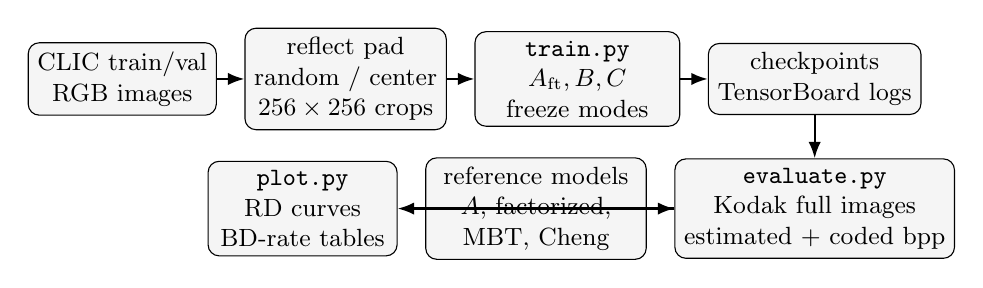
\begin{tikzpicture}[
  node distance=0.55cm and 0.35cm,
  pipe/.style={draw, rounded corners, align=center, minimum height=0.9cm, fill=gray!8},
  arr/.style={-{Latex[length=2.1mm]}, thick},
  font=\small
]
\node[pipe, minimum width=2.3cm] (clic) {CLIC train/val\\RGB images};
\node[pipe, right=of clic, minimum width=2.5cm] (patches) {reflect pad\\random / center\\\(256\times256\) crops};
\node[pipe, right=of patches, minimum width=2.6cm] (train) {\texttt{train.py}\\\(A_{\mathrm{ft}},B,C\)\\freeze modes};
\node[pipe, right=of train, minimum width=2.3cm] (ckpt) {checkpoints\\TensorBoard logs};
\node[pipe, below=of ckpt, minimum width=2.6cm] (eval) {\texttt{evaluate.py}\\Kodak full images\\estimated + coded bpp};
\node[pipe, left=of eval, minimum width=2.8cm] (refs) {reference models\\\(A\), factorized,\\MBT, Cheng};
\node[pipe, left=of refs, minimum width=2.4cm] (plots) {\texttt{plot.py}\\RD curves\\BD-rate tables};

\draw[arr] (clic) -- (patches);
\draw[arr] (patches) -- (train);
\draw[arr] (train) -- (ckpt);
\draw[arr] (ckpt) -- (eval);
\draw[arr] (refs) -- (eval);
\draw[arr] (eval) -- (plots);
\end{tikzpicture}
\caption{Final repository pipeline. The report uses the corrected Kodak evaluation path with actual entropy coding and the latest 2026-05-28 result summaries.}
\label{fig:pipeline}
\end{figure}

\section{Experiments}
\subsection{Experimental Setup}
The main project comparison uses the four Kodak operating points corresponding to qualities 1--4. We report PSNR, MS-SSIM, and coded bits per pixel. The fair comparison point is the fine-tuned vanilla baseline \(A_{\mathrm{ft}}\), not the frozen official pretrained model \(A\), because \(B\) and \(C\) are themselves fine-tuned from pretrained weights.

The repository also evaluates four stronger pretrained reference models from the CompressAI zoo: the factorized prior baseline, MBT 2018 mean, MBT 2018, and Cheng 2020 anchor. These are not direct baselines for the project hypothesis, but they help calibrate the size of any improvement. If a small SE block only changes BD-rate by a few hundredths of a percent while stronger priors improve it by 8--25\%, that strongly affects the interpretation of the result.

One important repository finding is that older intermediate results should not be used for the final report. The current \texttt{results\_discussion.md} explicitly notes that earlier plots were misleading because they mixed stale summaries and uncoded evaluation. The final report therefore uses the corrected summaries generated on 2026-05-28 by \texttt{evaluate.py} and \texttt{plot.py}.

\subsection{Main Rate-Distortion Results}
Figure~\ref{fig:rd-curves} shows the PSNR rate-distortion curves. The project zoom plot makes the main outcome clear: the curves for \(A_{\mathrm{ft}}\), \(B\), and \(C\) almost overlap. Across all four operating points, the maximum spread among these three models is below \(0.009\) dB and below \(5.8\times 10^{-4}\) bpp. This is too small to support a strong claim that the SE modification improved compression.

\begin{figure}[t]
\centering
\begin{subfigure}{\linewidth}
  \centering
  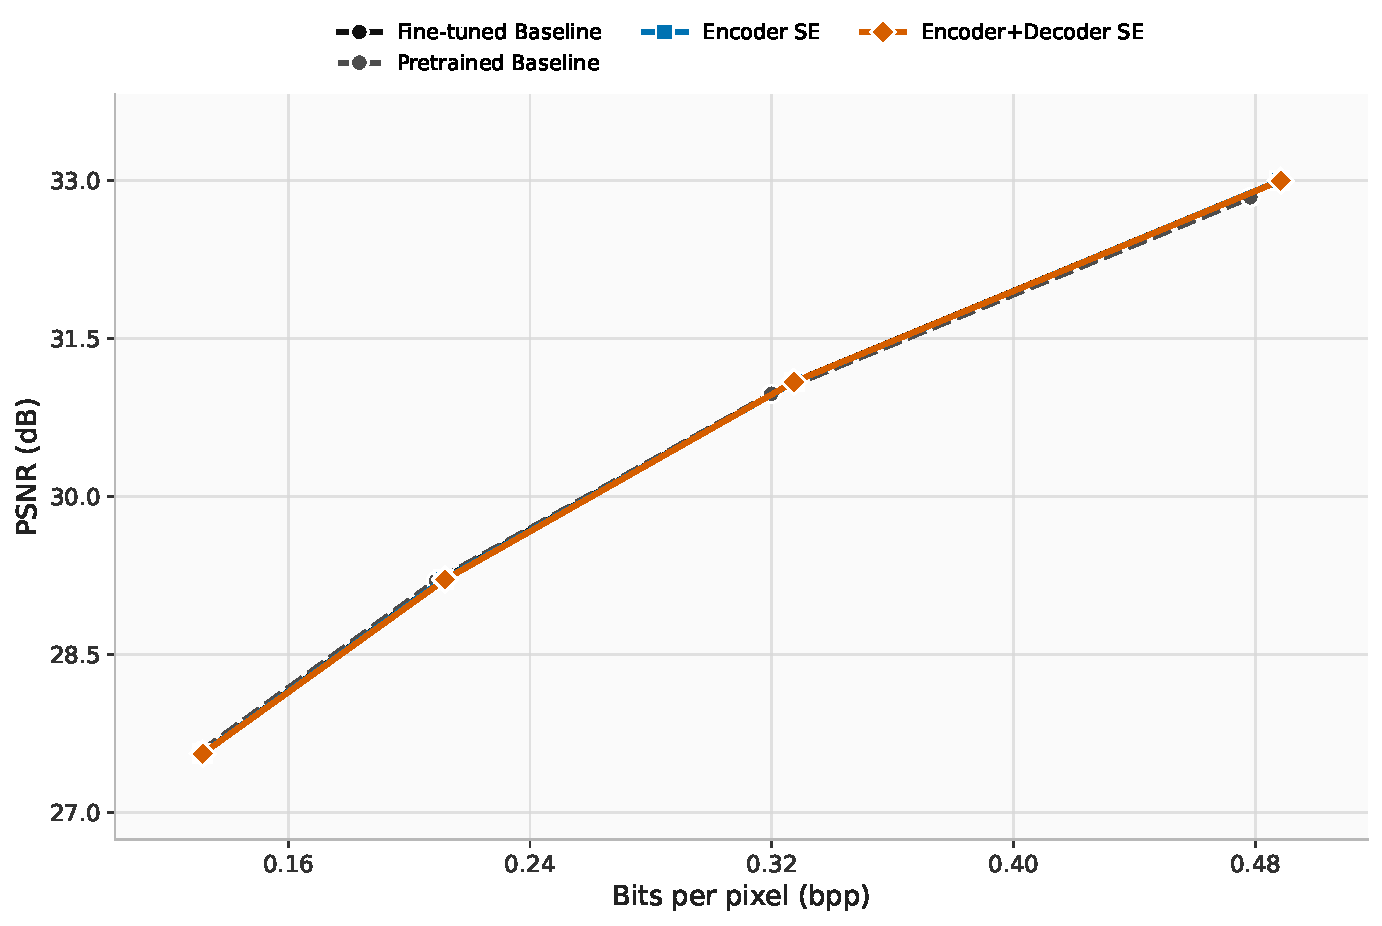
\includegraphics[width=\linewidth]{rd_curve_psnr_project_zoom.pdf}
  \caption{Project variants only.}
\end{subfigure}

\vspace{0.5em}

\begin{subfigure}{\linewidth}
  \centering
  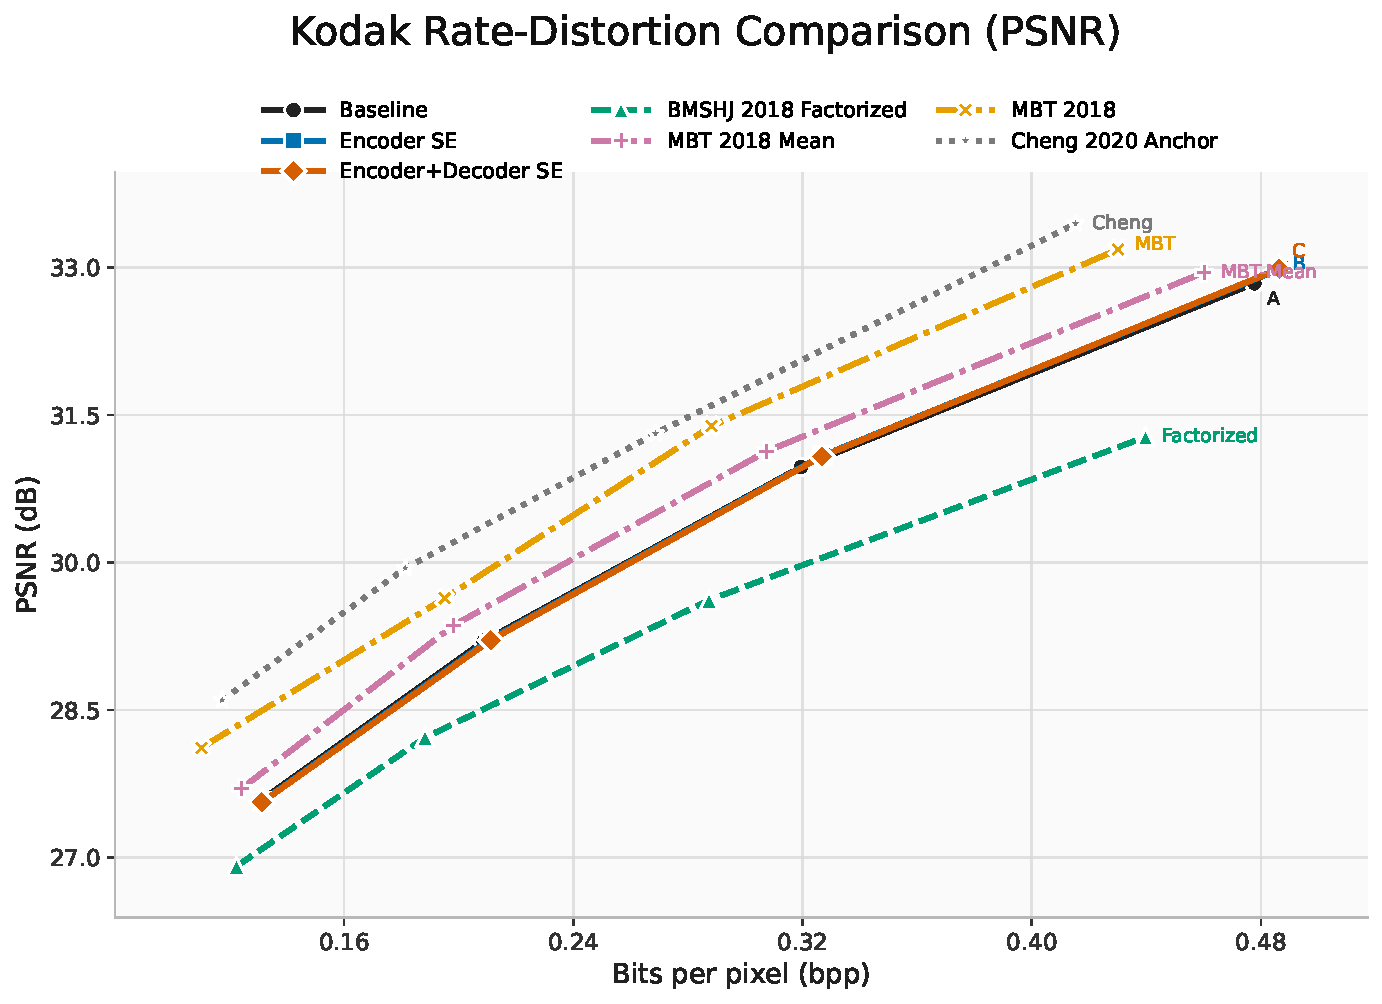
\includegraphics[width=\linewidth]{rd_curve_psnr.pdf}
  \caption{Project variants plus pretrained reference models.}
\end{subfigure}
\caption{PSNR rate-distortion curves on Kodak using coded bpp. The project variants are nearly indistinguishable, while stronger reference priors move the curve more substantially.}
\label{fig:rd-curves}
\end{figure}

Table~\ref{tab:bd-rate} quantifies this overlap through BD-rate relative to \(A_{\mathrm{ft}}\). The encoder-only SE model \(B\) is slightly worse in PSNR BD-rate and marginally better in MS-SSIM BD-rate; the encoder+decoder model \(C\) is slightly worse in both metrics. In practice, these numbers are so small that they should be interpreted as a tie rather than a meaningful gain. By contrast, MBT 2018 and Cheng 2020 provide clearly better RD behavior, which is consistent with the literature on stronger context and prior modeling.

\begin{table}[t]
\centering
\small
\caption{BD-rate relative to the fine-tuned vanilla baseline \(A_{\mathrm{ft}}\). Negative is better.}
\label{tab:bd-rate}
\begin{tabularx}{\linewidth}{@{}l c S[table-format=+2.2] S[table-format=+2.2]@{}}
\toprule
Model & {Params (M)} & {PSNR BD-rate (\%)} & {MS-SSIM BD-rate (\%)} \\
\midrule
Pretrained baseline \(A\) & 5.076 & -0.11 & -1.62 \\
Encoder SE \(B\) & 5.078 & +0.08 & -0.15 \\
Encoder+decoder SE \(C\) & 5.080 & +0.17 & -0.05 \\
BMSHJ 2018 factorized & 2.998 & +22.23 & +1.45 \\
MBT 2018 mean & 7.028 & -8.02 & -7.53 \\
MBT 2018 & 14.130 & -19.42 & -15.56 \\
Cheng 2020 anchor & 11.833 / 26.599 & -24.87 & -20.61 \\
\bottomrule
\end{tabularx}
\end{table}

The presence of \(A\) in Table~\ref{tab:bd-rate} is also informative. It is slightly better than \(A_{\mathrm{ft}}\), which suggests that local fine-tuning on the adopted CLIC setup did not improve the official pretrained model very much. This makes the negative result on SE attention easier to understand: the baseline itself is already strong, and the transform-side modification is small.

\subsection{Lightweight Parameter and Runtime Tradeoff}
The SE modification was intended to be lightweight, so it is important to check not only BD-rate but also parameter count and runtime. Table~\ref{tab:runtime-tradeoff} reports average Kodak timing across the four operating points for the main project comparison. The key observation is that the parameter overhead is indeed negligible: variant \(B\) adds only \(0.043\%\) parameters over \(A_{\mathrm{ft}}\), and variant \(C\) adds \(0.086\%\). Forward-pass latency is also close, with a \(1.44\%\) increase for \(B\) and a \(2.33\%\) increase for \(C\) relative to \(A_{\mathrm{ft}}\).

The codec-side timings tell a slightly more nuanced story. Variant \(B\) remains essentially tied with \(A_{\mathrm{ft}}\), but it is modestly slower overall (\(+1.57\%\) total encode+decode time). Variant \(C\) is again very close and in this rerun is slightly faster than \(A_{\mathrm{ft}}\) (\(-1.17\%\) total codec time), mainly because its average decode time is a bit lower. Given how small these differences are, the safest claim is not that SE improves speed, but that the SE additions do not impose a meaningful runtime penalty in the tested setup. Combined with the BD-rate table, this supports a clear conclusion: the modification is lightweight in both parameter count and wall-clock behavior, but it still does not buy a measurable compression gain.

\begin{table}[t]
\centering
\small
\caption{Lightweight tradeoff for the main project variants, averaged over Kodak qualities 1--4. Timings come from the corrected 2026-05-28 evaluation pipeline; forward pass is timed on GPU, while \texttt{compress()}/\texttt{decompress()} are timed on CPU.}
\label{tab:runtime-tradeoff}
\begin{tabularx}{\linewidth}{@{}l S[table-format=1.3] S[table-format=+1.3] S[table-format=2.2] S[table-format=2.2] S[table-format=2.2] S[table-format=3.2] S[table-format=+1.2]@{}}
\toprule
Variant & {Params (M)} & {Param \(\Delta\) (\%)} & {Forward ms} & {Encode ms} & {Decode ms} & {Codec total ms} & {Codec \(\Delta\) (\%)} \\
\midrule
\(A_{\mathrm{ft}}\) & 5.076 & 0.000 & 11.39 & 73.34 & 92.85 & 166.18 & 0.00 \\
\(B\) & 5.078 & +0.043 & 11.56 & 74.95 & 93.84 & 168.79 & +1.57 \\
\(C\) & 5.080 & +0.086 & 11.66 & 73.05 & 91.20 & 164.25 & -1.17 \\
\bottomrule
\end{tabularx}
\end{table}

\subsection{Freeze-Mode Ablations}
The freeze-mode ablations are scientifically useful because they test whether SE blocks act as effective adapters. Table~\ref{tab:freeze-ablation} reports the mid-rate operating point (\(\lambda=0.0067\), quality 3), where differences are easiest to inspect without extreme low- or high-rate behavior.

\begin{table}[t]
\centering
\small
\caption{Mid-rate ablation at quality 3 (\(\lambda=0.0067\)). Best epoch is read from the saved checkpoint metadata.}
\label{tab:freeze-ablation}
\begin{tabularx}{\linewidth}{@{}l l S[table-format=1.4] S[table-format=2.3] S[table-format=3.0]@{}}
\toprule
Variant & Freeze mode & {coded bpp} & {PSNR (dB)} & {Best epoch} \\
\midrule
\(A_{\mathrm{ft}}\) & none & 0.3279 & 31.094 & 86 \\
\(A_{\mathrm{ft}}\) & frozen hyperprior & 0.3276 & 31.092 & 84 \\
\(B\) & attention only & 0.3203 & 30.976 & 14 \\
\(B\) & none & 0.3276 & 31.087 & 77 \\
\(B\) & frozen hyperprior & 0.3268 & 31.075 & 87 \\
\(C\) & attention only & 0.3222 & 30.995 & 36 \\
\(C\) & none & 0.3273 & 31.086 & 93 \\
\(C\) & frozen hyperprior & 0.3275 & 31.080 & 68 \\
\bottomrule
\end{tabularx}
\end{table}

Two patterns stand out. First, \texttt{attention\_only} peaks much earlier and underperforms the fully trainable runs, especially for \(B\). This suggests that the SE modules alone do not have enough capacity to retune the compression model meaningfully. Second, \texttt{frozen\_hyperprior} is usually close to \texttt{none} but not better, so freezing the prior does not reveal a hidden benefit of the transform-side attention either.

Figure~\ref{fig:convergence} shows the validation curves for the \texttt{none} runs at quality 3. The three models converge in almost the same region, which matches the final Kodak evaluation. There is no visible sign that the SE variants settle at a distinctly better optimum.

\begin{figure}[t]
\centering
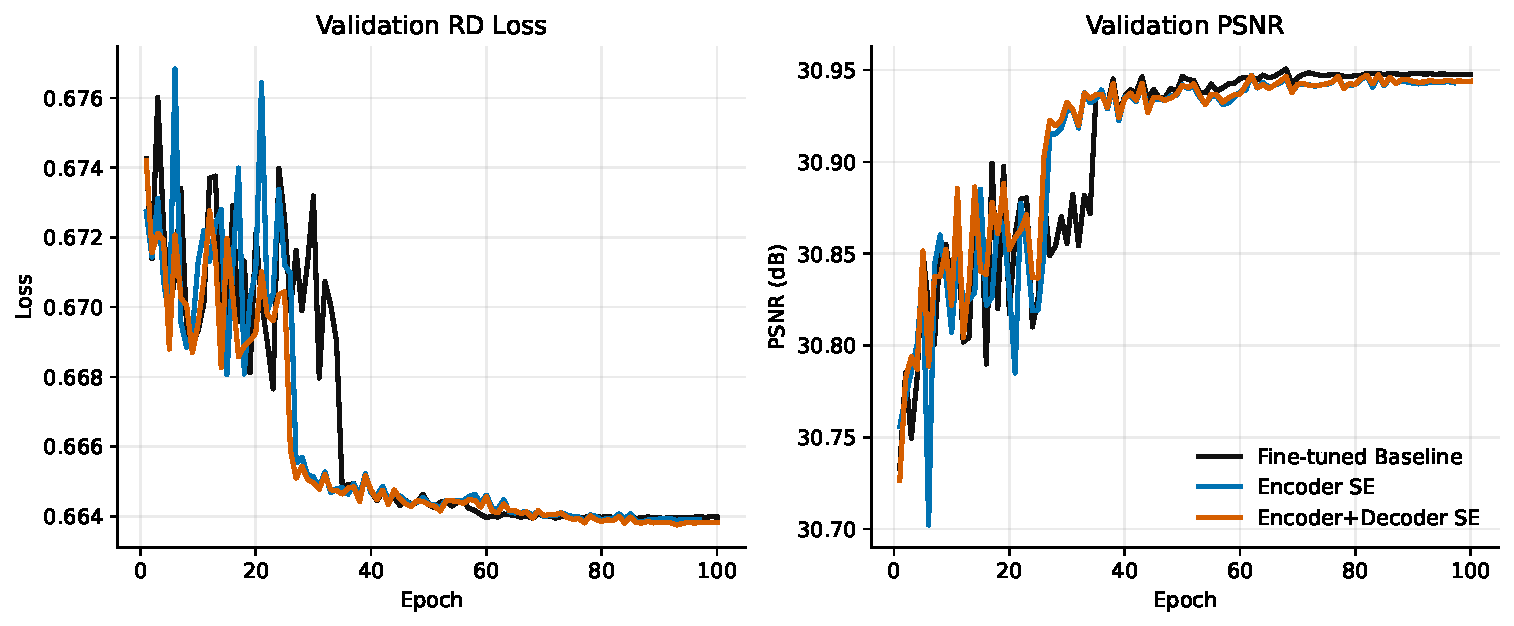
\includegraphics[width=\linewidth]{convergence_q3_none.pdf}
\caption{Validation convergence at quality 3 for the fully trainable runs. The curves track each other closely, and the final PSNR values are nearly identical.}
\label{fig:convergence}
\end{figure}

\subsection{Qualitative Reconstruction Comparison}
Figure~\ref{fig:qualitative} shows one Kodak example and a zoomed crop. All three project variants reconstruct the image well at the chosen operating point, but the differences among them are visually minor. The main artifacts are the same across models: slight smoothing around the printed text on the hat, softened fabric texture, and mild blur along edges.

\begin{figure}[t]
\centering
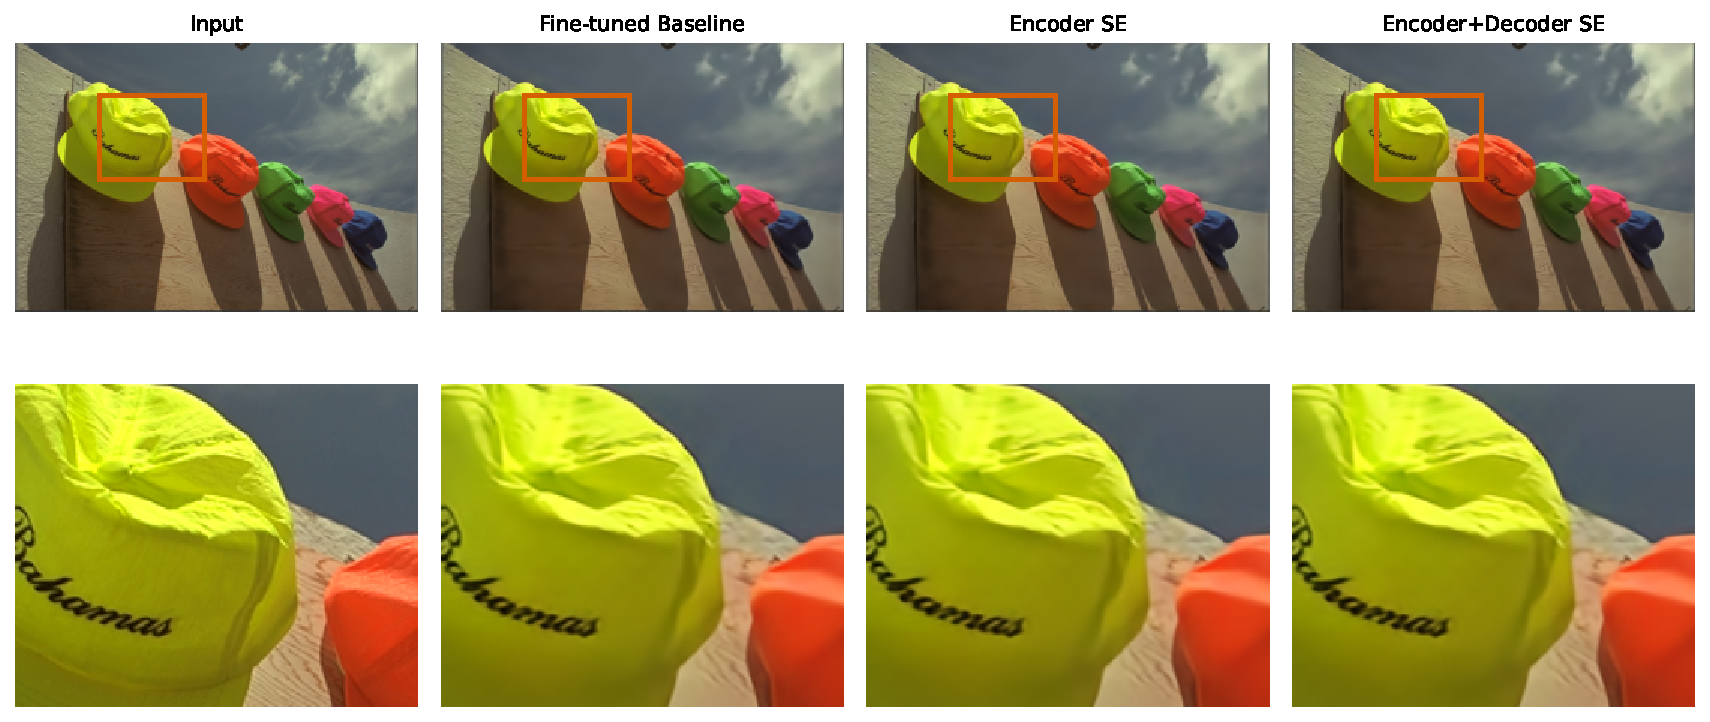
\includegraphics[width=\linewidth]{reconstruction_panel_q3_kodim03.pdf}
\caption{Qualitative comparison on Kodak image \texttt{kodim03} at quality 3. The SE variants do not recover clearly sharper structure than the fine-tuned vanilla baseline.}
\label{fig:qualitative}
\end{figure}

This qualitative result is consistent with the quantitative one. The SE blocks do not fail catastrophically; they simply do not produce a visible gain large enough to stand out from ordinary run-to-run or operating-point differences.

\subsection{What Is Missing and What Would Improve the Evidence}
Although the repository is in a reasonably good state for a term project, the experimental evidence is still limited in several ways.

\begin{itemize}[leftmargin=1.3em]
  \item Only one random seed is reported. Since the observed differences are extremely small, multi-seed training would be necessary to decide whether the tiny BD-rate gaps are real.
  \item All learned variants are trained with MSE. Training a parallel MS-SSIM-optimized set would make the MS-SSIM evaluation more meaningful.
  \item There is no classical codec baseline such as JPEG, JPEG 2000, or BPG. Even a limited comparison would improve the practical framing.
  \item Runtime is measured only on one local hardware/software stack. The current timing table is useful for relative comparison, but a stronger systems claim would require repeated measurements across multiple runs and cleaner CPU/GPU benchmarking conditions.
  \item The project changes only one SE insertion location. A broader attention-placement ablation could test whether the null result is due to weak attention or simply the chosen location.
\end{itemize}

Within the current repository, however, the central conclusion is already stable: stronger entropy models matter much more than the tested SE augmentation.

\section{Conclusion}
This project implemented the proposed idea successfully at the engineering level. We built two SE-augmented variants of the scale hyperprior, transferred pretrained weights carefully, added fair control baselines, trained multiple freeze-mode ablations, and evaluated the models with true coded bitrate on Kodak.

The final experimental outcome is negative but informative. After correcting the evaluation pipeline and comparing against a fine-tuned vanilla control, the SE variants do not provide a meaningful rate-distortion improvement. Their Kodak curves are essentially on top of the baseline, while stronger pretrained priors such as MBT 2018 and Cheng 2020 show clearly larger gains. The main lesson is that for learned compression, improving the prior model is usually more impactful than inserting a very small amount of channel attention into the transforms.

For a course project, this is still a useful result. The implementation work was substantial, the comparisons are reasonably clean, and the report can make an honest claim: under this training and evaluation setup, lightweight SE attention did not noticeably improve a scale-hyperprior image compressor.

\section*{Supplementary Suggestions}
The following supplementary material would strengthen the final submission without changing the main claims:

\begin{itemize}[leftmargin=1.3em]
  \item A short appendix with full per-image Kodak metrics and the coded-vs-estimated bitrate differences.
  \item A zip file containing the TensorBoard logs for the final 2026-05-28 runs.
  \item A small README describing the role of the main training, evaluation, plotting, and model files.
  \item Additional reconstruction panels or an interactive slider for \(A_{\mathrm{ft}}\), \(B\), and \(C\).
  \item If time permits before submission, an extra appendix table with multi-seed means and standard deviations.
\end{itemize}

\begin{thebibliography}{9}

\bibitem{balle2017e2e}
Johannes Ball\'e, Valero Laparra, and Eero P. Simoncelli.
\newblock End-to-end optimized image compression.
\newblock In \emph{International Conference on Learning Representations}, 2017.

\bibitem{balle2018hyperprior}
Johannes Ball\'e, David Minnen, Saurabh Singh, Sung Jin Hwang, and Nick Johnston.
\newblock Variational image compression with a scale hyperprior.
\newblock In \emph{International Conference on Learning Representations}, 2018.

\bibitem{hu2018senet}
Jie Hu, Li Shen, and Gang Sun.
\newblock Squeeze-and-excitation networks.
\newblock In \emph{Proceedings of the IEEE Conference on Computer Vision and Pattern Recognition}, pages 7132--7141, 2018.

\bibitem{minnen2018joint}
David Minnen, Johannes Ball\'e, and George Toderici.
\newblock Joint autoregressive and hierarchical priors for learned image compression.
\newblock In \emph{Advances in Neural Information Processing Systems}, volume 31, 2018.

\bibitem{cheng2020anchor}
Zhengxue Cheng, Heming Sun, Masaru Takeuchi, and Jiro Katto.
\newblock Learned image compression with discretized Gaussian mixture likelihoods and attention modules.
\newblock In \emph{Proceedings of the IEEE/CVF Conference on Computer Vision and Pattern Recognition}, pages 7939--7948, 2020.

\bibitem{begaint2020compressai}
Jean B\'egaint, Fabien Racap\'e, Simon Feltman, and Akshay Pushparaja.
\newblock CompressAI: a PyTorch library and evaluation platform for end-to-end compression research.
\newblock \emph{arXiv preprint arXiv:2011.03029}, 2020.

\bibitem{timofte2017div2k}
Radu Timofte, Eirikur Agustsson, Luc Van Gool, Ming-Hsuan Yang, and others.
\newblock NTIRE 2017 challenge on single image super-resolution: dataset and study.
\newblock In \emph{Proceedings of the IEEE Conference on Computer Vision and Pattern Recognition Workshops}, pages 114--125, 2017.

\bibitem{clic}
Workshop and Challenge on Learned Image Compression (CLIC).
\newblock \url{https://www.compression.cc/}. Accessed May 2026.

\bibitem{kodak}
Kodak Lossless True Color Image Suite.
\newblock \url{https://r0k.us/graphics/kodak/}. Accessed May 2026.

\end{thebibliography}

\end{document}
